\documentclass[12pt,a4paper]{article}
\renewcommand{\baselinestretch}{1.5} 
\usepackage[latin1]{inputenc}
\usepackage{amsmath}
\usepackage{amsfonts}
\usepackage{amssymb}
\usepackage{algorithm} 
\usepackage{algpseudocode} 
\usepackage{graphicx}
\usepackage{geometry}
\usepackage{tabulary}
\usepackage{caption}
\usepackage{subcaption}
\usepackage{xcolor}
\usepackage{dirtytalk}
\usepackage{bm}
\usepackage{longtable}
\usepackage{comment}
%\usepackage{ulem}
\graphicspath{{./images/}}

\usepackage[hyphens]{url}
%\usepackage{url}
% Toggle comment for hyperlinking the TOC and references
%\usepackage{hyperref}
%\hypersetup{
%	colorlinks=false%, % make the links colored
%	%linkcolor=blue, % color TOC links in blue
%	%urlcolor=red, % color URLs in red
%	%linktoc=all % 'all' will create links for everything in the TOC
%}

\geometry{
	left=2.5cm,
	right=2.5cm,
	top=2.5cm,
	bottom=3cm,
	}
	
	
	\usepackage{titlesec}
	
	\setcounter{secnumdepth}{4}
	\setcounter{tocdepth}{4}
	\titleformat{\paragraph}
	{\normalfont\normalsize\bfseries}{\theparagraph}{1em}{}
	\titlespacing*{\paragraph}
	{0pt}{3.25ex plus 1ex minus .2ex}{1.5ex plus .2ex}
	
	\newenvironment{conditions}
	{\par\vspace{\abovedisplayskip}\noindent\begin{tabular}{>{$}l<{$} @{${}={}$} l}}{\end{tabular}\par\vspace{\belowdisplayskip}}
	
	
		
\begin{document}
% uncomment title page when required to be included,
	\input{titlepage}
%%%%%%%%%%%%%%%%%%%%%%%%%%%%%%%%%%%%%%%%%%
	\pagenumbering{gobble}
	\renewcommand*\contentsname{Table of Contents}
	\tableofcontents
	\newpage
	\newpage
    \newpage
   % \newpage
   % \listoftables
    % \newpage
    \pagenumbering{arabic}
   
    \section{Introduction}
        Parallel computing enables multiple computations to execute simultaneously, improving performance over sequential execution. With the rise of multi-core processors, efficient scheduling of tasks has become essential to fully utilize available resources.

This project presents a parallel task scheduling simulator that models tasks using a Directed Acyclic Graph (DAG) and evaluates different scheduling algorithms based on performance metrics such as makespan, utilization, load imbalance, and speedup.

Parallel computing has become a fundamental paradigm in modern computing systems due to the increasing demand for high-performance applications such as scientific simulations, big data analytics, artificial intelligence, and real-time processing systems.

With the evolution of multi-core and many-core architectures, efficient utilization of computational resources has become a critical challenge. Task scheduling plays a central role in ensuring that workloads are distributed effectively across processors while minimizing execution time and maximizing resource utilization.

In real-world systems, tasks often exhibit dependencies, meaning certain tasks cannot begin execution until others have completed. These dependencies significantly constrain parallel execution and make scheduling more complex. Therefore, intelligent scheduling strategies are required to balance competing objectives such as minimizing makespan, reducing idle time, and maintaining load balance.

This project aims to address these challenges by simulating a DAG-based scheduling environment and evaluating multiple classical and heuristic scheduling algorithms. The study focuses not only on performance comparison but also on understanding how system parameters such as task size, processor count, and dependency density influence scheduling efficiency.
	\pagenumbering{arabic} 


	\subsection{Background}
	% write your Backgroud 
		In parallel systems, tasks are distributed across multiple processors for execution. However, dependencies between tasks restrict execution order and limit achievable parallelism.

These dependencies are modeled using a Directed Acyclic Graph (DAG), where nodes represent tasks and edges represent precedence constraints.

Efficient scheduling ensures that processors remain utilized while respecting these constraints.



		\subsection{Introduction to Problem Statement}
		Task scheduling in parallel systems is a complex problem due to task dependencies and varying execution times. Poor scheduling leads to increased makespan, processor idle time, and load imbalance.

The objective of this project is to simulate task scheduling using multiple algorithms and analyze their effectiveness in improving system performance.



		
	 %    \begin{figure}[h!]
		% 	\centering
		% 	\includegraphics[width=0.95\linewidth]{"Figure1"}
		% 	\caption{Give the Caption of Figure} 
		% 	\label{fig:figure-1}
		% \end{figure}
		
%     If You want too write bullet points
% These steps are:
    
%     \begin{itemize}
%         \item Some points one
%         \item[1.] another point 
%         \item some more points
%         \item Training the model on the datasets and revising it as required
%         \item Implementation of the model to generate results or outcomes.
%     \end{itemize}
    

    
	%	This goes to new chapter %\chapter
	\newpage
% 	\section{Literature Review}
	
	
% 	\begin{longtable}[htp]{|p{2cm}|p{2.5cm}|p{2.5cm}|p{3cm}|p{3.5cm}|}
% \caption{Summary of Literature Review}
% \label{Table1}
% \hline \textbf {References} & \textbf{Concepts} & \textbf{Technique(s)} & \textbf{Contribution} & \textbf{Limitations} \\
% \hline

% \cite{topcuoglu} & DAG Scheduling & HEFT Algorithm & Efficient task scheduling using priority ranking & Requires accurate execution time estimation \\

% \hline
% \cite{braun} & Task Mapping & Min-Min, Max-Min & Comparison of heuristic scheduling methods & Limited adaptability to dynamic workloads \\

% \hline
% \cite{kwok} & Parallel Scheduling & Static scheduling & Comprehensive survey of scheduling techniques & Limited focus on real-time performance \\

% \hline
% \end{longtable}

\section{Literature Review}

Task scheduling in parallel and distributed systems has been extensively studied due to its critical impact on system performance. Various algorithms have been proposed to optimize metrics such as makespan, resource utilization, and load balancing.

One of the most widely used approaches is the HEFT (Heterogeneous Earliest Finish Time) algorithm proposed by Topcuoglu et al. \cite{topcuoglu}. This algorithm ranks tasks based on their upward rank and assigns them to processors that minimize earliest completion time. While HEFT achieves good performance, it assumes accurate estimation of execution and communication costs, which may not always be realistic.

Braun et al. \cite{braun} conducted a comprehensive comparison of eleven static scheduling heuristics, including Min-Min and Max-Min algorithms. Their study highlighted that Min-Min performs well for smaller tasks by prioritizing tasks with minimum execution time, whereas Max-Min attempts to reduce starvation by prioritizing larger tasks. However, both approaches suffer from load imbalance under certain workload distributions.

Kwok and Ahmad \cite{kwok} provided a detailed survey of static scheduling algorithms for DAG-based task graphs. Their work emphasized the importance of considering precedence constraints and highlighted the computational complexity associated with optimal scheduling.

Classical scheduling theory, as discussed by Graham \cite{graham} and Coffman \cite{coffman}, provides foundational insights into multiprocessor scheduling and its inherent challenges. These works establish that optimal scheduling is NP-hard, necessitating the use of heuristic and approximation-based approaches.

Blazewicz et al. \cite{blazewicz} and Sinnen \cite{sinnen} further explored scheduling techniques in parallel systems, focusing on both theoretical models and practical implementations. Their studies emphasize the trade-off between scheduling optimality and computational overhead.

Recent research has also explored dynamic scheduling techniques that adapt to runtime conditions. Ahmad and Kwok \cite{ahmad} investigated task duplication strategies to reduce communication delays, while Li \cite{li} proposed methods to minimize processor idle time by improving task allocation strategies.

Despite these advancements, existing approaches often focus on optimizing a single performance metric, such as makespan, while neglecting load balancing and utilization. 


	
%	%\chapter
	\newpage
\section{Research Gaps}

Despite extensive research in parallel task scheduling, several challenges remain unaddressed.

First, many studies focus on evaluating algorithms under limited configurations, often ignoring variations in task size, processor count, and dependency density. This limits the generalizability of results.

Second, visualization of performance metrics is often underutilized. Graphical analysis provides intuitive insights into algorithm behavior, yet many works rely solely on numerical comparisons.

Third, load balancing is frequently overlooked as a primary optimization objective. While minimizing makespan is important, uneven workload distribution can lead to inefficient resource utilization.

Additionally, most existing approaches assume static environments where task characteristics are known in advance. Real-world systems, however, are dynamic and require adaptive scheduling strategies.

This project aims to bridge these gaps by:
\begin{itemize}
\item Evaluating multiple algorithms under diverse configurations
\item Incorporating graphical performance analysis
\item Introducing a load-aware scheduling strategy
\item Analyzing trade-offs between different performance metrics
\end{itemize}




%	%\chapter
	\newpage
	\section{Problem Formulation}

Let $T = \{t_1, t_2, \dots, t_n\}$ be a set of tasks.

Each task has:
\begin{itemize}
\item Execution time $e_i$
\item Dependency set $D_i$
\end{itemize}
The objective is to schedule these tasks on $P$ processors such that:
\begin{itemize}
\item Makespan is minimized
\item Dependencies are satisfied
\item Load is balanced across processors
\end{itemize}
Since optimal scheduling is NP-hard, heuristic-based algorithms are used.

\subsection*{Constraints and Assumptions}

The following assumptions are considered in this model:

\begin{itemize}
\item All processors are homogeneous in nature
\item Each processor can execute only one task at a time
\item Communication cost between tasks is ignored
\item Tasks are non-preemptive once assigned
\end{itemize}

\subsection*{Objective Optimization}

The scheduling problem aims to minimize the makespan while maintaining load balance:

\[
\min \; M = \max(C_i)
\]

Additionally, the system aims to minimize load imbalance:

\[
LI = \frac{\max(load) - \min(load)}{\text{average load}}
\]
%	
%	
	\section{Objectives}

The primary objective of this project is to design and analyze an efficient task scheduling system for parallel computing environments using Directed Acyclic Graph (DAG) models.

The specific objectives of this work are as follows:

\begin{itemize}

\item To design and implement a parallel task scheduling simulator capable of handling task dependencies using DAG representation.

\item To study and implement multiple classical scheduling algorithms such as FCFS, Round Robin, Min-Min, and Max-Min.

\item To develop a custom Load-Aware scheduling algorithm that dynamically assigns tasks based on processor workload.

\item To evaluate and compare the performance of different scheduling algorithms using standard metrics such as makespan, utilization, speedup, and load imbalance.

\item To analyze the impact of varying system parameters, including task size, processor count, and dependency density, on scheduling performance.

\item To ensure efficient utilization of computational resources by minimizing processor idle time.

\item To study the trade-offs between different scheduling strategies in terms of performance and computational complexity.

\item To visualize and interpret experimental results using graphical representations for better understanding.

\item To investigate the scalability of scheduling algorithms as the number of tasks and processors increases.

\item To identify limitations of existing scheduling techniques and propose improvements through load-aware strategies.

\item To provide a flexible and extensible simulation framework that can be adapted for future research in parallel and distributed computing.

\end{itemize}
	
	
	\section{Methodology}

The proposed system simulates a parallel task scheduling environment using a Directed Acyclic Graph (DAG). The workflow consists of the following steps:

\begin{itemize}
\item Task generation with random execution times
\item Creation of task dependencies forming a DAG
\item Selection of scheduling algorithm
\item Assignment of tasks to processors
\item Parallel execution using OpenMP
\item Calculation of performance metrics
\item Storage of results in CSV format
\item Visualization using graphs
\end{itemize}

\subsection*{System Architecture}

The system is designed as a modular simulation framework consisting of the following components:

\begin{itemize}
\item \textbf{Task Generator:} Generates tasks with random execution times and dependencies.
\item \textbf{DAG Constructor:} Builds a Directed Acyclic Graph representing task relationships.
\item \textbf{Scheduler Module:} Implements various scheduling algorithms.
\item \textbf{Execution Engine:} Simulates parallel execution using OpenMP.
\item \textbf{Metrics Calculator:} Computes performance metrics such as makespan, utilization, speedup, and load imbalance.
\item \textbf{Visualization Module:} Generates graphs for analysis.
\end{itemize}

\begin{figure}[h]
\centering
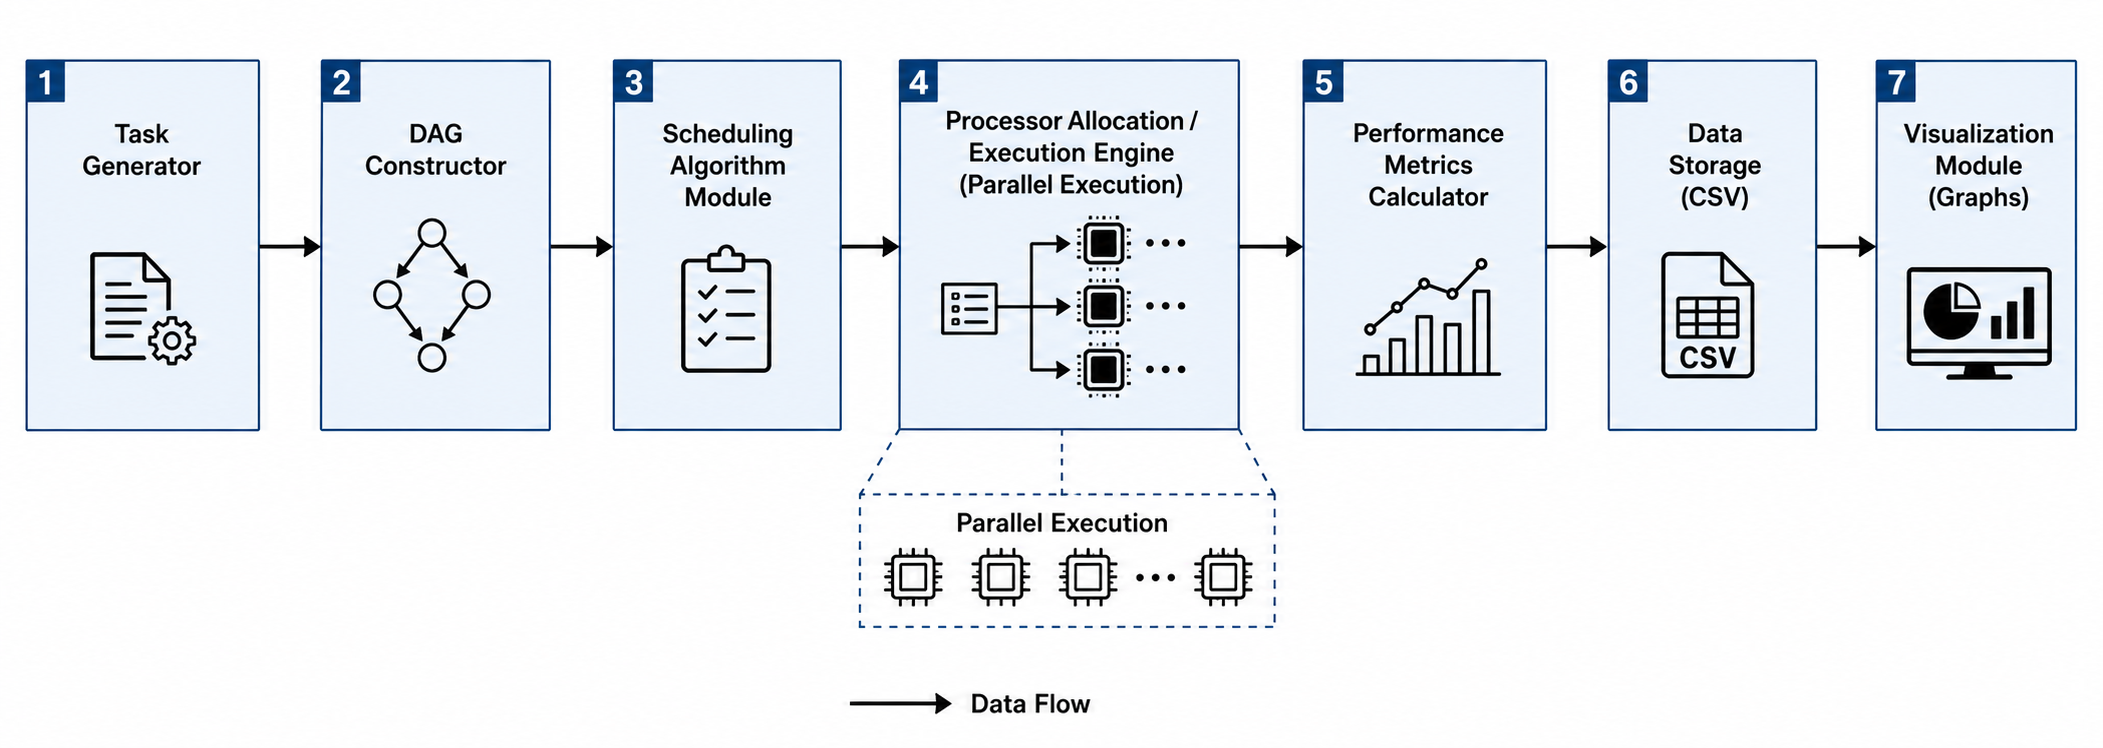
\includegraphics[width=1\linewidth]{dag_layers.png}
\caption{Example of a layered Directed Acyclic Graph (DAG) representing task dependencies}
\label{fig:dag}
\end{figure}

\subsection*{Working Principle}

The simulation begins with task generation, followed by DAG construction. Scheduling algorithms are then applied to assign tasks to processors. Tasks are executed in parallel while respecting dependencies. Finally, performance metrics are computed and stored for analysis.

This modular design allows easy integration of additional scheduling algorithms and scalability for larger experiments.

\subsection{Scheduling Algorithms}

The following algorithms are implemented:

\begin{itemize}
\item FCFS (First Come First Serve)
\item Round Robin
\item Min-Min
\item Max-Min
\item Load-Aware (custom algorithm)
\end{itemize}

\begin{algorithm}
\caption{Parallel Task Scheduling Simulator}
\begin{algorithmic}[1]
\State Generate tasks with execution time and dependencies
\State Construct DAG
\For{each scheduling algorithm}
    \State Initialize processors
    \While{tasks remain}
        \State Select ready tasks (no pending dependencies)
        \State Assign tasks to processors
        \State Execute tasks in parallel
    \EndWhile
    \State Compute metrics (makespan, utilization, speedup)
\EndFor
\end{algorithmic}
\end{algorithm}

\subsubsection{Load-Aware Scheduling (Proposed)}

The Load-Aware scheduling algorithm is a custom heuristic designed to improve load balancing across processors.

The algorithm assigns each task to the processor with the minimum current workload. At each step, ready tasks are selected and assigned dynamically based on processor load.

\textbf{Steps:}
\begin{itemize}
\item Identify ready tasks
\item Calculate current load on each processor
\item Assign task to least loaded processor
\item Update processor load
\end{itemize}
\textbf{Advantages:}
\begin{itemize}
\item Minimizes load imbalance
\item Improves processor utilization
\item Reduces makespan
\end{itemize}
\textbf{Limitation:}
It is a greedy approach and does not consider future task dependencies or critical path.

\begin{figure}[h]
\centering
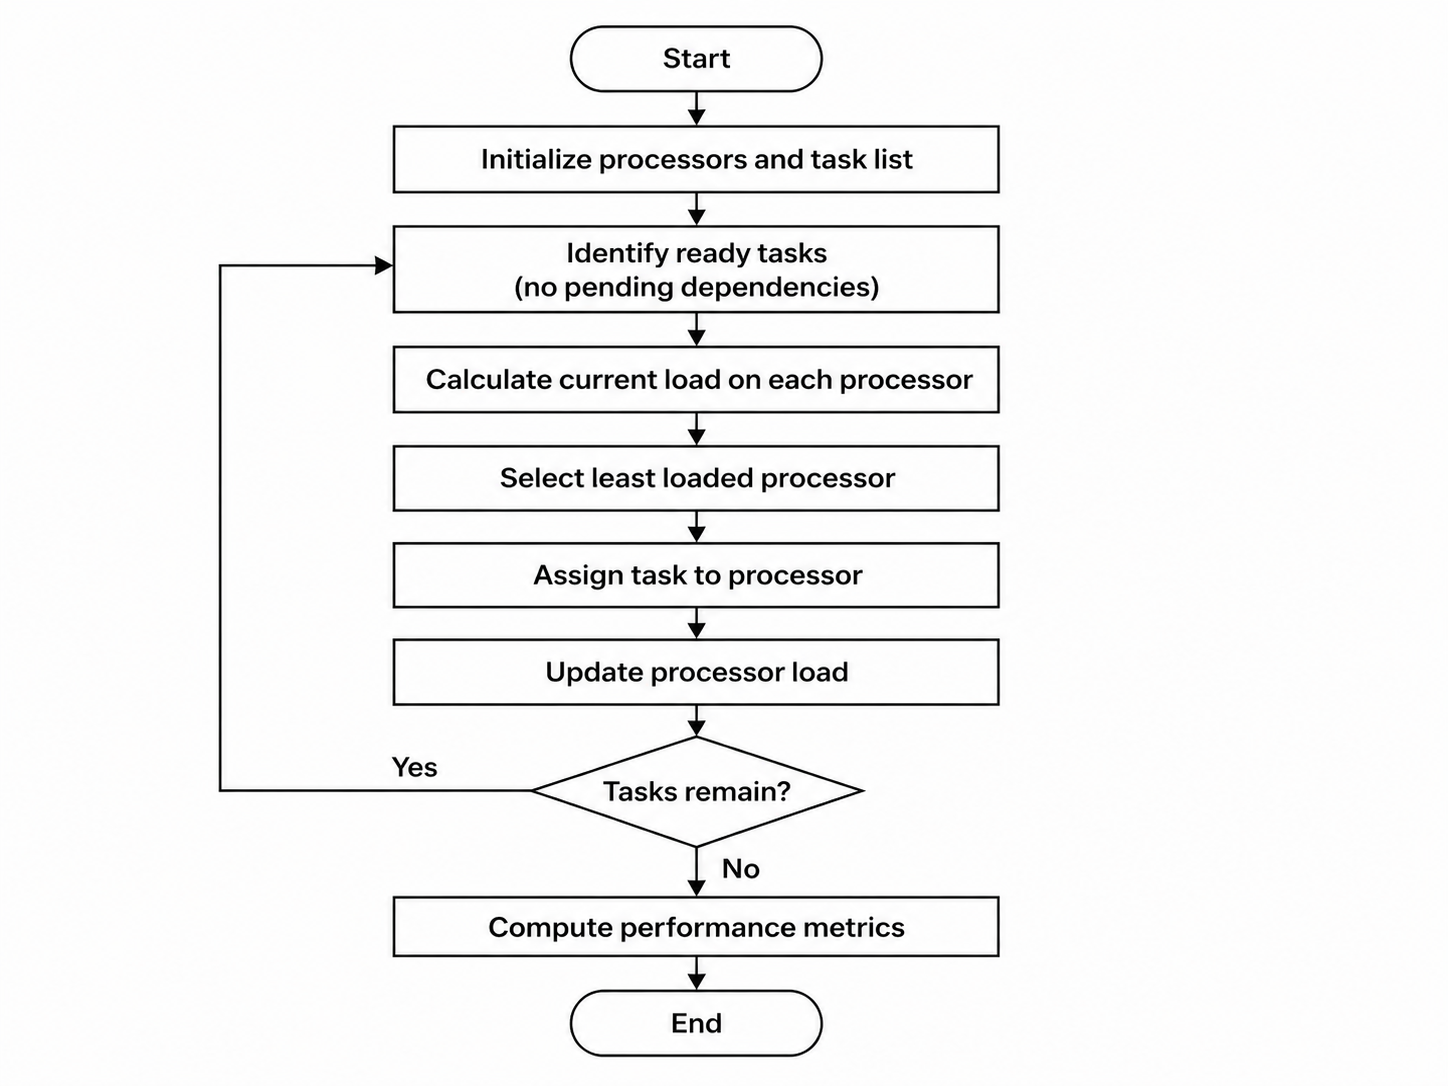
\includegraphics[width=0.76\linewidth]{load-aware.png}
\caption{Flowchart of the proposed Load-Aware scheduling algorithm}
\label{fig:loadaware}
\end{figure}

\subsection{Equation}
The following performance metrics are used:

\textbf{Makespan:}
\[
M = \max_{i}(finish\_time_i)
\]

\textbf{Utilization:}
\[
U = \frac{\sum busy\_time_i}{P \times M}
\]

\textbf{Speedup:}
\[
S = \frac{T_{sequential}}{T_{parallel}}
\]

\textbf{Load Imbalance:}
\[
LI = \frac{max\_load - min\_load}{average\_load}
\]
 
 
    
   %\chapter
   \newpage
  \section{Datasets}

This project uses synthetically generated task datasets.

Each task is characterized by:
\begin{itemize}
\item Execution time (random between 1 and 50 units)
\item Dependencies on previous tasks
\end{itemize}

Experiments are conducted using:
\begin{itemize}
\item Task sizes: 50, 100, 200
\item Number of processors: 2, 4, 8
\end{itemize}
This setup allows evaluation of scalability and performance under different workloads.
The dataset is generated randomly to simulate real-world task scheduling scenarios.

The dependency probability is set to 20\%, meaning each task has a 20\% chance of depending on previous tasks. This ensures the formation of a realistic DAG structure.
\subsection*{Dataset Characteristics}

The dataset used in this project is synthetically generated to simulate realistic scheduling scenarios.

Each task is assigned a random execution time within a predefined range, ensuring variability in workload. Dependencies are introduced probabilistically to create a DAG structure that mimics real-world applications such as workflow systems and scientific computations.

The use of synthetic datasets allows controlled experimentation, enabling analysis of how different parameters affect scheduling performance. By varying task size and processor count, the scalability of algorithms can be evaluated effectively.

Multiple runs are conducted for each configuration to ensure consistency and reduce the impact of randomness. The results are averaged to provide reliable performance metrics.


   \newpage
%    \section{Results and Discussion}

% \begin{figure}[h]
% \centering
% 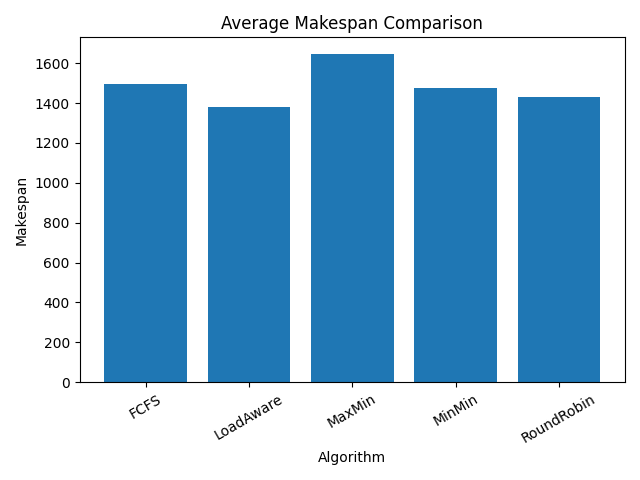
\includegraphics[width=0.7\linewidth]{makespan.png}
% \caption{Makespan Comparison}
% \end{figure}

% \begin{figure}[h]
% \centering
% 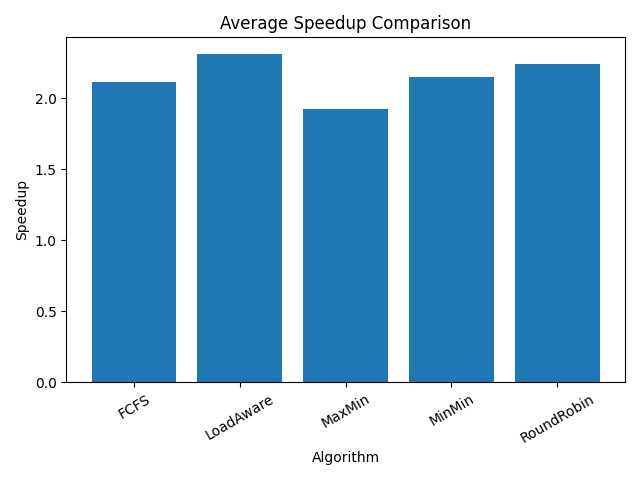
\includegraphics[width=0.7\linewidth]{speedup.png}
% \caption{Speedup Comparison}
% \end{figure}

% \begin{figure}[h]
% \centering
% 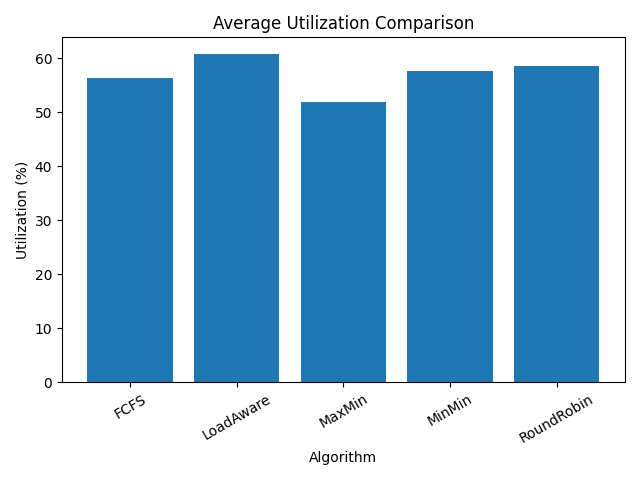
\includegraphics[width=0.7\linewidth]{utilization.png}
% \caption{Utilization Comparison}
% \end{figure}

\section{Results and Discussion}

\begin{figure}[h]
\centering

\begin{subfigure}{0.32\linewidth}
    \centering
    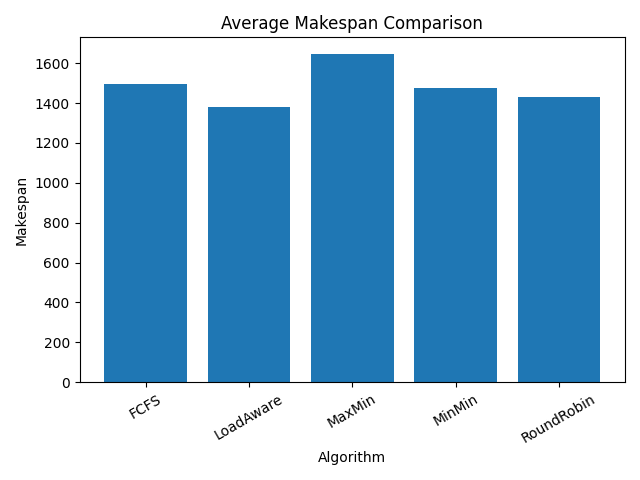
\includegraphics[width=\linewidth]{makespan.png}
    \caption{Makespan}
\end{subfigure}
\hfill
\begin{subfigure}{0.32\linewidth}
    \centering
    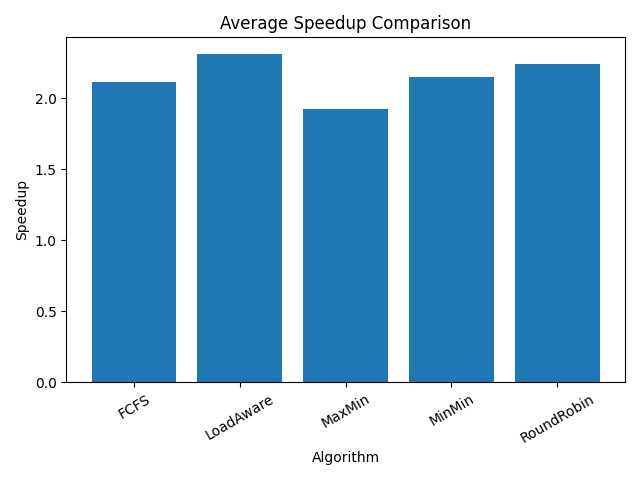
\includegraphics[width=\linewidth]{speedup.png}
    \caption{Speedup}
\end{subfigure}
\hfill
\begin{subfigure}{0.32\linewidth}
    \centering
    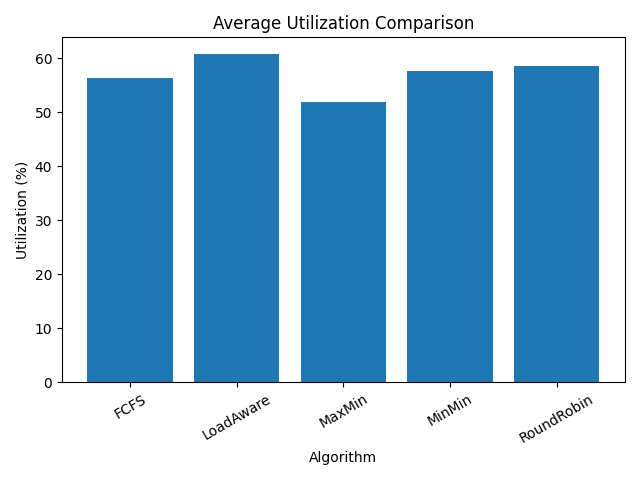
\includegraphics[width=\linewidth]{utilization.png}
    \caption{Utilization}
\end{subfigure}

\caption{Comparison of scheduling algorithms based on makespan, speedup, and utilization across multiple configurations}
\end{figure}

It is observed that Load-Aware achieves the lowest makespan and load imbalance, while Max-Min shows the worst performance. Round Robin maintains stable performance across all configurations.

\subsection{Observations}

The experiments were conducted under varying configurations:

\begin{itemize}
\item Task sizes: 50, 100, 200
\item Processors: 2, 4, 8
\item Execution time range: 1--50
\item Dependency probability: 20\%
\end{itemize}
Further, the experiments show that:
\begin{itemize}

\item Increasing processors from 2 to 8 reduces makespan but decreases utilization due to idle processors.

\item Increasing task size increases makespan but improves utilization.

\item Load imbalance is lowest in Load-Aware scheduling (as low as 0.02), while Max-Min shows highest imbalance (up to 3.7).

\item Speedup increases with processors but is limited due to task dependencies.

\end{itemize}




% \begin{figure}[h]
% \centering
% 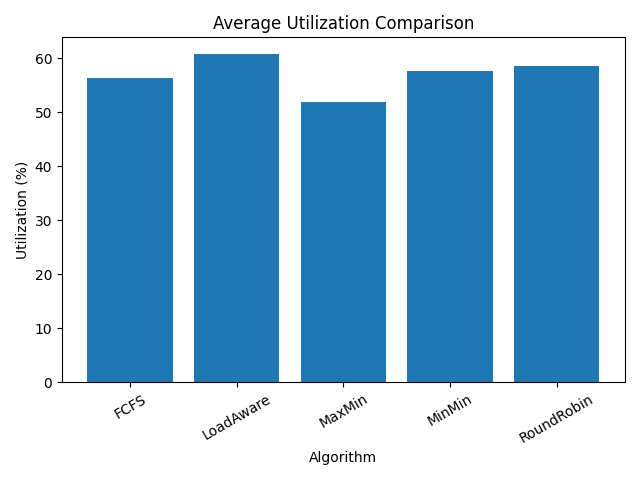
\includegraphics[width=0.7\linewidth]{utilization.png}
% \caption{Utilization Comparison}
% \end{figure}
\begin{table}[h]
\centering
\caption{Best Performing Algorithm per Metric}
\begin{tabular}{|c|c|}
\hline
Metric & Best Algorithm \\
\hline
Makespan & Load-Aware \\
Utilization & Load-Aware \\
Load Imbalance & Load-Aware \\
Speedup & Load-Aware / Round Robin \\
\hline
\end{tabular}
\end{table}

\subsection*{Interpretation of Results}

The results clearly demonstrate that scheduling performance is highly dependent on both algorithm design and system configuration.

The Load-Aware algorithm consistently outperforms others due to its dynamic workload distribution strategy. By assigning tasks to the least loaded processor, it minimizes idle time and improves overall efficiency.

Round Robin shows stable performance across all configurations, indicating its robustness. However, it does not achieve optimal results due to lack of dependency awareness.

Min-Min performs well for smaller workloads but struggles as task size increases. This is because it tends to prioritize short tasks, leading to delays in executing longer tasks.

Max-Min exhibits the poorest performance, as prioritizing large tasks often results in underutilization of processors.

These findings highlight the importance of balancing multiple objectives rather than optimizing a single metric.

\subsection{Detailed Analysis}

From the experimental results, the following trends are observed:

\begin{itemize}

\item \textbf{Load-Aware Algorithm:} 
Consistently achieves the lowest makespan and lowest load imbalance. This is due to its dynamic load balancing strategy.

\item \textbf{Round Robin:}
Provides stable performance with moderate makespan and low imbalance due to equal distribution.

\item \textbf{Min-Min:}
Performs well for smaller tasks but suffers when larger tasks dominate.

\item \textbf{Max-Min:}
Shows the worst performance due to prioritization of large tasks, leading to idle processors.

\end{itemize}

\begin{table}[h]
\centering
\caption{Average Performance Comparison}
\begin{tabular}{|c|c|c|c|c|}
\hline
Algorithm & Makespan & Utilization (\%) & Load Imbalance & Speedup \\
\hline
FCFS & 1324 & 59.2 & 1.36 & 2.20 \\
RoundRobin & 1243 & 62.1 & 0.29 & 2.35 \\
MinMin & 1306 & 59.0 & 0.93 & 2.24 \\
MaxMin & 1435 & 54.2 & 2.45 & 2.05 \\
LoadAware & 1208 & 63.7 & 0.25 & 2.42 \\
\hline
\end{tabular}
\end{table}

\subsection*{Time Complexity Analysis}

The scheduling complexity depends on the number of tasks (n) and processors (p).

\begin{itemize}
\item FCFS: O(n)
\item Round Robin: O(n)
\item Min-Min / Max-Min: O(n^2)
\item Load-Aware: O(n log p)
\end{itemize}

The Load-Aware algorithm provides a balance between efficiency and performance improvement.

\subsection*{Limitations}

The study has the following limitations:

\begin{itemize}
\item Synthetic datasets may not fully represent real-world workloads
\item The Load-Aware algorithm does not consider critical path optimization
\item Communication cost between processors is not modeled
\item Assumes homogeneous processors
\end{itemize}

\newpage
\section{Conclusion}

The experimental results demonstrate that the Load-Aware algorithm consistently outperforms traditional scheduling techniques in terms of makespan, utilization, and load balancing.

The results also highlight that increasing the number of processors improves speedup but reduces utilization due to idle resources. Task dependencies significantly limit parallel performance, aligning with theoretical expectations such as Amdahl{’}s Law.

Overall, the study validates the effectiveness of load-balanced scheduling strategies in parallel computing systems.

\subsection*{Future Scope}

Future work can extend this study in several directions.

One potential improvement is the implementation of dynamic scheduling algorithms that adapt to real-time system conditions. Additionally, incorporating machine learning techniques for predictive scheduling can further enhance performance.

The system can also be extended to distributed computing environments using frameworks such as MPI or cloud-based platforms. This would enable evaluation under more realistic conditions.

Another direction is to consider heterogeneous systems where processors have varying capabilities, introducing additional complexity to the scheduling problem.

Finally, integrating energy efficiency as a performance metric can provide a more comprehensive evaluation of scheduling algorithms.
	% to add references to TOC without section numbering
%	%\chapter
	\newpage
	\begin{thebibliography}{99}

\bibitem{topcuoglu}
H. Topcuoglu, S. Hariri, and M. Wu, “Performance-effective and low-complexity task scheduling for heterogeneous computing,” IEEE Transactions on Parallel and Distributed Systems, 2002.

\bibitem{braun}
T. D. Braun et al., “A comparison of eleven static heuristics for mapping a class of independent tasks onto heterogeneous distributed computing systems,” Journal of Parallel and Distributed Computing, 2001.

\bibitem{kwok}
Y. Kwok and I. Ahmad, “Static scheduling algorithms for allocating directed task graphs to multiprocessors,” ACM Computing Surveys, 1999.

\bibitem{graham}
R. L. Graham, “Bounds on multiprocessing timing anomalies,” SIAM Journal on Applied Mathematics, 1969.

\bibitem{coffman}
E. G. Coffman Jr., “Computer and Job-Shop Scheduling Theory,” Wiley, 1976.

\bibitem{blazewicz}
J. Blazewicz, K. Ecker, E. Pesch, G. Schmidt, and J. Weglarz, “Scheduling in Computer and Manufacturing Systems,” Springer, 1994.

\bibitem{sinnen}
O. Sinnen, “Task Scheduling for Parallel Systems,” Wiley-Interscience, 2007.

\bibitem{ahmad}
I. Ahmad and Y. Kwok, “On exploiting task duplication in parallel program scheduling,” IEEE Transactions on Parallel and Distributed Systems, 1998.

\bibitem{li}
K. Li, “Scheduling precedence constrained tasks with reduced processor idle time,” IEEE Transactions on Parallel and Distributed Systems, 2012.

\bibitem{dongarra}
J. Dongarra et al., “A set of level 3 basic linear algebra subprograms,” ACM Transactions on Mathematical Software, 1990.

\end{thebibliography}

  
     \end{document}
%        
%       